\chapter{Volume Penalty}
\label{ch:Volume Penalty}

Our method ensures that volume is preserved within each zone, but without any element-wise volume
change penalty the volume inside each zone can transfer between elements. This is a feature, as discussed in the Introduction, since
it reduces the cost and numerical challenges of enforcing volume preservation locally, while
ensuring good behavior globally.  Note that, unlike in the hydrostatic case, volume can not transfer
completely freely since elastic forces due to the shear modulus restrict large flows. 

\new{
	However, the zonal constraints by themselves model only the hydrostatic pressure in the coarse zones, hence we need to also model the finer-scale pressures in the individual elements.
	We employ a more traditional approach to modeling element-wise pressure by using a penalty method.
	To model this penalty function, we look at the volume penalty functions present in Neo-Hookean elasticity models.
	In Neo-Hookean models, the bulk modulus models how much the material resists volumetric deformation per element. 
	The bulk moudulus is represented in most Neo-Hookean energy formulations in the first Lam\'e parameter $\lambda$, which is a combination of the shear and bulk modulus.
	However, as discussed in Section~\ref{sec:back}, when $\lambda \rightarrow +\infty$ locking occurs, and the pressure computations become unstable.
	But since we model the coarse-scale pressures as constraints, and we only need to model the finer-scale deviations in pressures, we are able to use a lower $\lambda$ and avoid locking.
}

If $\lambda$ is set too low the simulation is more susceptible to collapsing elements 
and even equilibrium configurations with inverted elements for invertible energy models.
Consider the example in Figure~\ref{fig:pucks} of a cylindrical puck with a moving Dirichlet
boundary condition on a set of vertices on top of the puck. As the puck compresses, the tetrahedra
underneath the moving boundary are flattened to the point where subsequent steps cause boundary
adjacent tetrahedra to invert. At this point, incompressible energy models with a logarithmic volume
penalty ($\log J$) term will become undefined because $J \leq 0$. Other models, like co-rotated
elasticity, may permit inverted elements, but won't be able to recover from an inverted
configuration. This issue has motivated a number of solutions \cite{Irving:2004,Smith:2018} for
handling inverted elements, but we will focus on the recent work on the Stable Neo-Hookean
model developed by Smith et al. While the proposed model attempts to solve many of the issues with
non-invertible energies and doesn't require additional parameters, as can be seen from the plot
of the volume change penalty term in terms of relative volume change $J$ in Figure~\ref{fig:penalty_plots},
the Stable Neo-Hookean energy resists compression much more timidly as compared to
the standard Neo-Hookean model defined in Equation \eqref{eq:neohookean}.
\new{
	This results in the simulation possibly converging to an invalid configuration where inverted elements exist, 
	and a nonlinear optimization solver can struggle due to inverted elements being present in intermediate solutions and causing oscillations.
	Especially, this solver oscillations can be aggravated when constraints are introduced, presenting major performance issues when one tries to use volume constraints. 
}
%% TODO with new energy model
\begin{figure}[t] 
	\centering
	\begin{subfigure}{.49\linewidth}
		\centering 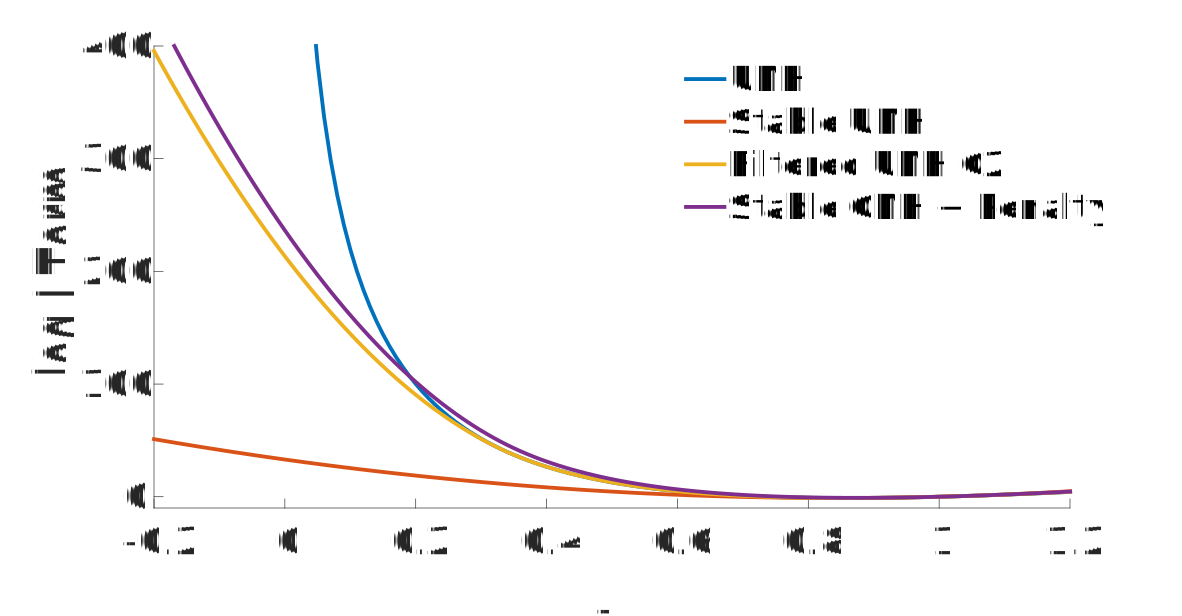
\includegraphics[width=1.5in]{images/energy_plot.pdf}
		\caption*{(a)}
		\label{sfig:energy_plot}
	\end{subfigure}%
	\begin{subfigure}{.49\linewidth}
		\centering \includegraphics[width=1.5in]{images/stress_plot.pdf}
		\caption*{(b)}
		\label{sfig:stress_plot}
	\end{subfigure}%
	\caption{\textbf{Penalty Plots}: A plot of the penalty terms $U(J)$ and their stresses $U'(J)$ from different
		energy formulations (Neo-Hookean, Stable Neo-Hookean \cite{Smith:2018}, the second-order expanded version of Stable Neo-hookean, \cite{kikuuwe:2009},
		ours with $\beta=1$, and ours with $\beta=6$) with $\lambda = 1$, in terms of the relative volume change $J$. 
		The Neo-Hookean volume term (blue) indicates a substantially larger penalty
		when compared to Stable Neo-Hookean (orange) 
		and \cite{kikuuwe:2009} (yellow), but the penalty term is undefined when $J \leq 0$ due to its log term.
		This is more evident to see in the stress plot during compression ($J < 1$), where the Stable
		Neo-Hookean volumetric stress changes in a linear manner. Our method for both $\beta=1$ (purple) and $\beta=6$ (green) shows much more effective penalization under compression and stretch. Our stresses shows a nonlinear dependence on $J$
		similar to the Neo-Hookean term, but also shows a effective growth not only during compression but also during stretch. }
	\label{fig:penalty_plots}
\end{figure}

This suggests a need for a good penalty term that is both invertible and still resists compression
effectively. Let us write such penalty term as $U(J)$, controlled linearly by parameter $\lambda$.
To design such a penalty term, we first take a look at what conditions the function $U(J)$ must
meet. 
\new{
	A detailed study of various Neo-Hookean volume penalty terms and explanations for each of the 
	conditions can be found in \cite{hartmann:2003}.
}

\begin{enumerate}[label=\alph*)]
	\item The function must evaluate to 0 at rest ($J = 1$).
	\item The gradient of the function, i.e the volumetric stress, must also evaluate to 0 at rest.
	\item For the $\lambda$ of the penalty term to  correspond to the Lam\'e parameter in linear elasticity, $\frac{\partial^2 U(1)}{\partial J^2} = 1$ must hold.
	\item The function must be defined for all real numbers $(-\infty, +\infty)$.
	\item $\frac{\partial^2 U(J)}{\partial J^2} \geq 0, \,\forall J \in \R$ for the penalty to both penalize compression and stretch.
\end{enumerate}

Consider the following function,
\begin{equation}
U(J; \beta) := \frac{1}{12} (J-1)^2 \left[ \beta (J-1)^2 + 6 \right],
\label{eq:penalty_function}
\end{equation}
where the parameter $\beta \in [0, +\infty)$ controls how steeply the penalty function will penalize change in $J$. 
The first and second derivatives of the function are 
\begin{align}
\frac{\partial U(J; \beta)}{\partial J} &= \frac{1}{3} (J-1) \left[ \beta (J-1)^2 + 3 \right], \text{ and}\\
\frac{\partial^2 U(J; \beta)}{\partial J^2} &= \beta (J-1)^2 + 1. 
\label{eq:penalty_derivatives}
\end{align}
Therefore, the function satisfies all of the conditions listed above.    
Note that for $\beta = 0$, $U(J;0) = U_{\text{SNH}}(J) = \frac{1}{2} (J-1)^2$. 
As $\beta$ is increases, the penalty function penalizes compression and stretch more effectively than the Stable
Neo-Hookean penalty term, while still being fully invertible. 
Therefore, this is a suitable choice for our compression penalty term.
Plots comparing different penalty terms $U(J)$ and stresses $\frac{\partial U(J)}{\partial J}$ are shown in Figure~\ref{fig:penalty_plots}.
Experimentally, $\beta = 1$ was sufficient for most realistic examples governed by external force, but for examples where inversions were more likely due to contact or boundary conditions, we could easily find higher $\beta$ that resolves all inversions.

\new{
	The additional nonlinearity introduced in the gradient (Equation \eqref{eq:penalty_derivatives}) of our penalty function compared to a standard Stable Neo-Hookean penalty is the main reason for the inversion-robustness in our model. 
	It is possible to formulate even more nonlinear models than what we propose here, but in our experiments we found that such energy models provide no significant benefit in resolving inversions compared to \eqref{eq:penalty_function} and only increase the number of nonlinear solver iterations until convergence.
}

We demonstrate that by this simple addition to the energy potential, we can obtain results similar to 
that of using mixed finite elements as in \cite{Irving:2007}, but with very few or even 
one global constraint. The results of Figure  \ref{fig:suspended-cubes} demonstrate
that with a penalty of about $\nu = 0.45$ and with just one global zone, the deformations are close to 
using a 1-ring constraint around each vertex. 
\new{
	Also, we found that simply adding this additional nonlinearity to the energy resulted in faster performances in most examples when volume constraint was used, and even in many cases where there were no constraints. 
	In Table~\ref{tab:performance}, we compare the performance results of using $\beta = 0$ (equivalent to SNH) and higher $\beta$.
}